% Vorlage für eine Bachelor- oder Masterthesis
%% Dipl.-Ing. Stefan Averkamp
%% Version 2.5
%% 18.03.2021
%% ----------------------------------------------------------------------------

\documentclass[
cmyk,
pdftex,
a4paper,           % DinA4 Papier
%12pt,             % Schriftgröße
oneside,           % oneside, twoside
openright,         % openleft, openright, openany
numbers=noenddot,  % keinen Punkt hnter Kapitel- oder Sectionnummern
chapterprefix=off, % Kapitel wird vor die Kapitelnummer geschrieben
]{scrbook}
%% Preambel einbinden -----------------------------------------------------------------------------
\UseRawInputEncoding
\setcounter{secnumdepth}{3}         % 3 levels in section numbering

%% Useful packages -------------------------------------------------------------------------------
\usepackage[english]{babel}         % English language
\usepackage{scrhack}
\usepackage{placeins}
\usepackage{subcaption}
\usepackage{lmodern}
\usepackage{cmbright}
\usepackage{enumitem}               % Package for customized lists
\usepackage[OT1]{fontenc}
\usepackage{blindtext}              % Use \blindtext to insert dummy text
\usepackage{mdwlist}                % More compact lists with itemize and co
\usepackage{graphicx}               % Graphics
\usepackage{epstopdf}               % Automatically convert eps images to pdf
\usepackage{ltxtable}               % Combines longtable and tabularx
\usepackage{multirow}               % Multi-row cells in tables
\usepackage[dvipsnames,table,xcdraw]{xcolor}  % Alternating colors in tables
\usepackage{rotating}               % Rotate text and other elements
\usepackage{multicol}               % Multicolumn formatting
\usepackage{amsmath}                % Mathematical formulas
\usepackage{amsthm}                 % Theorem style
\usepackage{mathtools}
\usepackage{amssymb}                % Mathematical symbols
\usepackage{wrapfig}                % Wrapping figures
\usepackage{float}                  % For [h!] or [H] positioning
\usepackage{booktabs}               % For tables from Excel to LaTeX
\usepackage{eurosym}                % Use Euro symbol
\usepackage{url}                    % URLs
\usepackage{etoolbox}
\appto\UrlBreaks{\do\a\do\b\do\c\do\d\do\e\do\f\do\g\do\h\do\i\do\j
    \do\k\do\l\do\m\do\n\do\o\do\p\do\q\do\r\do\s\do\t\do\u\do\v\do\w
    \do\x\do\y\do\z}
\usepackage{adjustbox}
\usepackage{fancybox}               % Boxes and frames
\usepackage{caption}                % Extended settings for captions
\usepackage{array}                  % Extended options for arrays and tables
\usepackage{icomma}                 % Reduces space after comma in decimal numbers
\usepackage{setspace}               % Define line spacing

%% PDF options (links and more) -----------------------------------------------------------------
\usepackage{pdfpages}
\usepackage[utf8]{inputenc}         % UTF-8 encoding
\usepackage[english=british]{csquotes}
\usepackage[pdftex, raiselinks, pdfpagelabels, hypertexnames=false, pdfstartview={Fit}]{hyperref}
\definecolor{lightblue}{rgb}{0.9,0.9,1}

%% PDF metadata
\hypersetup{
    pdfauthor = {Nico Bierbaum},
    pdftitle =  {Scientific Work},
    pdfsubject = {Density and Shrinkage Evaluation of 316L Printed Parts in the FDM Process},
    pdfkeywords = {3D printing, filament, metal, density, tensile test, shrinkage},
    pdfcreator = {LaTeX with hyperref package}
}

%% Header and footer -----------------------------------------------------------------------------
\usepackage[headsepline]{scrlayer-scrpage}
\pagestyle{scrheadings}
\clearpairofpagestyles
\ihead{\headmark} % Redefine
\ohead{\pagemark}

%% Page margins -----------------------------------------------------------------------------------
\usepackage[a4paper,inner=4cm,outer=2.5cm,top=2cm,bottom=2cm,includeheadfoot]{geometry}

%% Bibliography -----------------------------------------------------------------------------------
\usepackage[style=numeric-comp,sorting=none,backend=biber]{biblatex}

\DeclareFieldFormat{labelalpha}{\textsc{#1}}    % Sets the author in small caps 
\renewcommand*{\mkbibnamefamily}[1]{\textsc{#1}}  % Sets the last name in small caps 
\renewcommand*{\mkbibnamegiven}[1]{\textsc{#1}}  % Sets the first name in small caps 
\renewcommand*{\mkbibnameprefix}[1]{\textsc{#1}}  % Sets the prefix in small caps 
\DeclareFieldFormat{title}{``#1''}      % Sets the title in quotation marks
\DeclareFieldFormat{date}{({#1})}               % Sets the date in parentheses
\makeatletter
\def\blx@maxline{77}
\makeatother
\addbibresource{LiteratureDB.bib} % Load bibliography

%% Glossary and abbreviations ---------------------------------------------------------------------
\usepackage{nomencl}
% English title
\renewcommand{\nomname}{Glossary and List of Abbreviations}
% Dots between abbreviation and explanation
\setlength{\nomlabelwidth}{.20\hsize}
\renewcommand{\nomlabel}[1]{#1 \dotfill}
% Reduce line spacing
%\setlength{\nomitemsep}{-\parsep}
\makenomenclature
\setlength{\headsep}{1.5\baselineskip}

%% ---------------------------------------------------------------------------------------------------
%% Create glossary and abbreviations: ------------------------------------------------------------------
%% 1. Run LATEX
%% 2. Open a command prompt and navigate to the folder with the "thesis.tex" file.
%% 3. Run the command   makeindex thesis.nlo -s nomencl.ist -o thesis.nls
%% 4. Run LATEX again. The glossary and abbreviations should now be present.

%% Source code -------------------------------------------------------------------------------------
\usepackage{listings}
\lstset{ %
    basicstyle=\scriptsize,         % the size of the fonts that are used for the code
    numbers=left,                   % where to put the line-numbers
    numberstyle=\footnotesize,      % the size of the fonts that are used for the line-numbers
    backgroundcolor=\color{white},  % choose the background color. You must add \usepackage{color}
    commentstyle=\color{green},
    stringstyle =\color{orange},
    xleftmargin=1.5em,
    xrightmargin=1em,
    frame=tb,                       % adds a frame around the code
    tabsize=2,                      % sets default tabsize to 2 spaces
    captionpos=b,                   % sets the caption-position to top or bottom
    breaklines=true,                % sets automatic line breaking
    breakatwhitespace=false         % sets if automatic breaks should only happen at whitespace
    literate =%
     {#}{\#}1
}
\renewcommand*{\lstlistingname}{Source Code}
\renewcommand*{\lstlistlistingname}{List of Source Codes}

%% Tikz for (complex) colorful drawings ---------------------------------------------------------
\usepackage{tikz}
\usetikzlibrary{positioning,mindmap,shapes,shapes.multipart,shadows,arrows,patterns,topaths}
\usepackage{pgfplots}
\pgfplotsset{width=7cm,compat=newest}

\definecolor{yellow}{HTML}{FFFCCC}
\definecolor{green}{HTML}{CFFFCC}
\definecolor{blue}{HTML}{CCE9FF}
\definecolor{darkblue}{HTML}{99b7EE}
\definecolor{red}{HTML}{FFA8A8}
\definecolor{orange}{HTML}{FFD28F}

\lstset
{
    breaklines=true,
    tabsize=3,
    showstringspaces=false
}

\lstdefinestyle{Common}
{
    extendedchars=true,
    language={[Visual]Basic},
    frame=single,
    %===========================================================
    framesep=3pt,%expand outward.
    framerule=0.4pt,%expand outward.
    xleftmargin=3.4pt,%make the frame fits in the text area. 
    xrightmargin=3.4pt,%make the frame fits in the text area.
    %=========================================================== 
    rulecolor=\color{Red}
}

\lstdefinestyle{A}
{
    style=Common,
    backgroundcolor=\color{Yellow!10},
    basicstyle=\scriptsize\color{Black}\ttfamily,
    keywordstyle=\color{Orange},
    identifierstyle=\color{Cyan},
    stringstyle=\color{Red},
    commentstyle=\color{Green}
}

\lstdefinestyle{B}
{
    style=Common,
    backgroundcolor=\color{Black},
    basicstyle=\scriptsize\color{White}\ttfamily,
    keywordstyle=\color{Orange},
    identifierstyle=\color{Cyan},
    stringstyle=\color{Red},
    commentstyle=\color{Green}
}


\begin{document}

%% Titelseite einbinden ---------------------------------------------------------------------------
\thispagestyle{empty}
\newgeometry{
	top=25mm, 
	bottom=7mm,
	left=46mm,
	right=36mm
}
%Logos------------------------------------------------------------------------------
%Logos bekommen eine definierte Breite von 6cm, die Box in der das Logo ist, ist 7cm
\vspace*{-2cm} %evtl nützlich um logos weiter oben zu platzieren
\setlength{\unitlength}{1cm}
\hfill
%% Firmenlogo ----------------------------------------------------------------------
\begin{minipage}[t]{14cm}
\begin{minipage}[t]{7cm}

\end{minipage}
%% FH-Logo ----------------------------------------------------------------------
\begin{minipage}[t]{7cm}
   \begin{flushright}
    
\includegraphics[width=66mm]{bilder/fhm_Logo_CMYK_30mm.pdf}
   \end{flushright}
\end{minipage}\\
\end{minipage}
%-----------------------------------------------------------------------------------

\begin{minipage}[t]{11cm}
\vspace{2cm}					
\begin{Huge}
\begin{center}\textsf{\textbf{Wissenschaftliche Arbeit}}\end{center}
\end{Huge}


\vspace{2cm} 								
\begin{Large}
\hfill 
\begin{center}

\begin{large}
	Nico Bierbaum
\end{large}

\vspace{2cm} %3cm
%\begin{minipage}[t][2.5cm]{14cm}
\begin{flushright}
	\hfill{Analyse der Dichte und Schwindung sowie Ermittlung mechanischer Kennwerte von Edelstahlkomponenten, hergestellt mittels 3D-Druck im FDM-Verfahren}\\
\end{flushright}			
%\end{minipage}
\end{center}	
\end{Large}

\begin{large}
\vspace{30mm}  %3cm
%\begin{minipage}[t][1.5cm]{14cm}
\hfill Betreuer der Arbeit: Prof. Dr.-Ing. Hilmar Apmann

\hfill Steffen Florian M.Sc.\\
%\end{minipage}
\end{large}

\vspace{35mm}
\hfill Steinfurt, den \today
\end{minipage}
\vspace{20mm}

\begin{minipage}[t]{136.5mm}
\begin{flushright}

\includegraphics[width=82mm]{bilder/MB_CMYK.pdf}
\end{flushright}
\end{minipage}
\restoregeometry
%--------------------------------------------------------------------------------------------------------

%% Sperrvermerk, Eidesstattliche Erklärung, Vorwort -----------------------------------------------
\frontmatter

\pagestyle{scrheadings}
\pagenumbering{Roman}
%\input{inhalt/kapitel1.tex}

%\input{inhalt/Sperrvermerk.tex}				nicht notwenig???
%%Eidesstattliche Erklärung-------------------------------------------------------------------------------
\chapter*{Eidesstattliche Erklärung}
\addcontentsline{toc}{chapter}{Eidesstattliche Erklärung}

Ich erkläre hiermit an Eides statt, dass ich die vorliegende Hausarbeit selbstständig und ohne unzulässige fremde Hilfe angefertigt habe. Die verwendeten Literaturquellen sind im Literaturverzeichnis vollständig zitiert.





\vspace{6cm}
Steinfurt, \today
	nicht notwendig???
%% Vorwort -----------------------------------------------------------------------------------------
\chapter*{Vorwort}

Schreiben wir den Bums hier ein bisschen wie Werbung oder soll das komplett sachlich und nüchtern passieren?

\addcontentsline{toc}{chapter}{Vorwort}



%% Inhaltsverzeichnis einbinden -------------------------------------------------------------------
\pdfbookmark[0]{Inhaltsverzeichnis}{tableofcontents}
\tableofcontents

%% Verzeichnisse einbinden  -----------------------------------------------------------------------
\listoffigures              %% Abbildungsverzeichnis
\listoftables               %% Tabellenverzeichnis
%\lstlistoflistings          %% Quelltextverzeichnis
\nomenclature{AM}{Additive Fertigung \textit{engl. Additive Manufacturing}}
\nomenclature{CAD}{rechnerunterstütztes Konstruieren \textit{engl. Computer Aided Design}}
\nomenclature{FDM}{Schmelzschichten \textit{engl. Fused Deposit Modeling}}
\nomenclature{CNC}{rechnergestützte numerische Steuerung \textit{engl. Computer Numerical Control}}
\nomenclature{SLM}{selektives Laserschmelzen \textit{engl. Selective Laser Melting}}
\nomenclature{PTFE}{Polytetrafluorethylen}
\nomenclature{Heizblock}{Baugruppe aus Heizelement und Druckdüse}
\nomenclature{PLA}{Polylactide}
\nomenclature{PETG}{Polyethylenterephthalat}
\nomenclature{ABS}{Acrylnitril-Butadien-Styrol-Copolymer - Thermoplast}
\nomenclature{Firmware}{Software, die in elektronische Geräte fest implementiert ist}
\nomenclature{Open-Source}{Software, deren Quellcode frei verfügbar ist und von unabhängigen Dritten eingesehen und editiert werden kann}
\nomenclature{Software}{Begriff für Programme auf technischen Geräten}




\cleardoublepage% or \clearpage
\markboth{\nomname}{\nomname}

\printnomenclature
% \addcontentsline{toc}{chapter}{Glossar und Abkürzungsverzeichnis}
  %% Abkuerzungsverzeichnis
%% Eigentlicher Inhalt der Arbeit -----------------------------------------------------------------
%% Einbinden der einzelnen Kapitel. Jedes Kapitel in eine seperate Datei speichern. ---------------
\mainmatter

\chapter{Einleitung}
\label{einleitung}

\subsection*{Disclaimer zur Verwendung des generischen Maskulinums}
Für die Lesbarkeit und bessere Verständlichkeit dieses Businessplans haben wir uns dazu entschieden, das generische Maskulinum zu verwenden. Wir möchten darauf hinweisen, dass wir damit keinesfalls eine Diskriminierung oder Geringschätzung von Personen anderer Geschlechter beabsichtigen. Selbstverständlich sind alle im Text verwendeten Bezeichnungen geschlechtsneutral zu verstehen und gelten gleichermaßen für Frauen und Männer.

\pagebreak

\section{Hintergrund und Motivation}
Additive Fertigung \textit{engl. Additive Manufacturing (AM)} wurde in den 1990ern eingeführt und beschreibt eine bis dahin neuartige Technologie 3D-Objekte in einem Schicht-für-Schicht Verfahren zu fertigen. Im Gegensatz zur additiven Fertigung [AM] steht die subtraktive Fertigung, auch als konventionelle Fertigung bezeichnet. Bei der die gewünschten Bauteile durch Abtrag von Material (z.B. beim Fräsen oder Drehen) hergestellt werden. Durch die additive Fertigung ergibt sich eine hohe Flexibilität und Designfreiheit, dies ist insbesondere für Prototypenherstellung, als auch immer mehr in der Serienproduktion von Bedeutung \autocite{Prof.Dr.Ing.ChristianSeidel.2023}.
Zu Beginn ist diese Technologie hauptsächlich in der Prototypenphase eingesetzt, da sich die Materialienauswahl auf Polymere beschränkt. So gab es vor allem viele Kunststoffe zur Auswahl, aber keine Materialien, die einem Stahl gleichkommen.
Heute ist AM im weiteren Sinne auch für die Herstellung von funktionellen Teilen eingesetzt.  Firmen aus den Bereichen Luft- und Raumfahrt, Automobilherstellung, Energie und Medizin sind interessiert an dem Einsatz der AM zur Herstellung verschiedener Bauteile.
AM bringt folgende Vorteile mit sich:
\begin{itemize}
    \item Große Freiheit im Design der Bauteile, was eine individuelle Anpassung an die Produktion ermöglicht. Zudem ist die Erstellung komplexer Bauteile deutlich einfacher als mit konventionellen Methoden.
    \item Der Konstruktionsprozess und die Prototypenphase sind deutlich schneller. Einzelne Prozessschritte sind schneller.
\end{itemize}

1.1 Hintergrund und Motivation\\
1.2 Zielsetzung der Arbeit\\
1.3 Aufbau der Arbeit
\chapter{Theoretische Grundlagen}

Die additive Fertigung hat in den letzten Jahren Fortschritte gemacht und ist zu einem Bestandteil der modernen Fertigungstechnologie geworden. Innerhalb dieses Prozesses werden Bauteile über rechnerunterstütztes Konstruieren \textit{(engl. Computer Aided Design (CAD))} entworfen. Über Verfahren der additiven Fertigung werden diese Bauteile dann gefertigt. Der Druck mittels Schmelzschichten \textit{(engl. Fused Deposit Modeling (FDM))} hat sich als eine vielversprechende Methode etabliert, um komplexe dreidimensionale Objekte schichtweise aufzubauen. Während FDM-Druckverfahren traditionell auf Polymermaterialien ausgerichtet sind, hat die Weiterentwicklung dieser Technologie nun den Weg für den Einsatz von Metallfilamenten eröffnet \autocite{Osama2019}. In diesem Kapitel werden die theoretischen Grundlagen erläutert.

\section{Additive Fertigung und der FDM-Prozess}

AM wird als Verfahren bezeichnet, bei dem Materialien entweder durch Verschmelzung, Bindung oder Verfestigung von Materialien wie flüssigen Harzen und Pulvern gemischt werden. Im Gegensatz dazu stehen subtraktive Verfahren, die einen Abtrag von Material hervorrufen, wie zum Beispiel die rechnergestützte numerische Steuerung \textit{(engl. Computer Numerical Control (CNC))}. Bei additiven Verfahren wird das zuvor entwickelte 3D-Bauteil in einzelne Schichten unterteilt, um die gewünschte Geometrie zu erreichen. Diese Schichten werden aus einer Polygon-Datei generiert. Um alle Einstellungen zu treffen, wird eine spezielle Software verwendet. Hier ist auch ein essentieller Unterschied zur CNC-Fertigung, denn mithilfe dieser Software wird unter anderem die Auflösung des Bauteils vorgegeben, welches vor anderem Einflüsse auf die Fertigungszeit hat.\\
Der Begriff FDM wurde 1989 zuerst erwähnt und beschreibt das Prinzip bei dem Rohmaterial durch einer aufgeheizten Düse extrudiert wird. Die Extrusion wird auf ein spezielles Druckbett appliziert. Die Extrusion bildet Linien, welche dann aneinander gereiht eine Schicht ergibt. Alle Schichten aufeinander ergeben dann das fertige Bauteil. \autocite{Osama2019}

\subsection{Materialien für den FDM-Prozess}

Bisher werden meistens verschiedenste Kunststoffe, oder eine Mischung derer, für den FDM-Druck verwendet. Diese Arbeit beschäftigt sich darüber hinaus mit dem Druck von einem Metallfilament.

\subsection{316L-Edelstahl als Druckmaterial}

Obwohl der FDM-Druck vorwiegend für Kunststoffe verwendet wird, haben viele Firmen mit der Entwicklung von Metallfilamenten begonnen. Diese Filamente binden Metallpartikel in einem Polymer. Anders als beim selektiven Laserschmelzen \textit{engl. Selective Laser Melting (SLM)}, bei dem Metallpartikel mittels eines Lasers aufgeschmolzen werden, entstehen somit kein gefährlicher, aufgewirbelter Staub. SLM gehört ebenfalls zur Gruppe AM. \autocite{MetalAdditiveMan}
\begin{figure}[h]
	\centering
	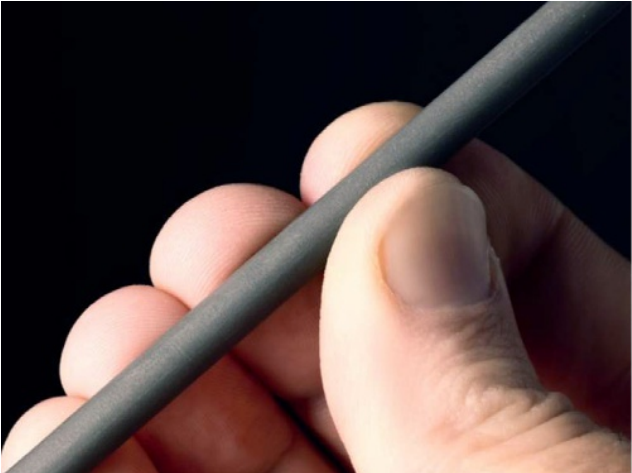
\includegraphics[width=0.5\linewidth]{bilder/Beispiel_Metallfilament.png}
        \caption[Beispiel für ein Metallfilament in Rohform] {Beispiel für ein Metallfilament in Rohform \autocite{MetalAdditiveMan}}
	\label{fig:FilamentBeispiel}
\end{figure}

Nachdem die gewünschte Kontur gefertigt ist, besteht sie weiterhin aus Metallpartikel gebunden mit Polymer. Damit dieses Polymer nun entweicht, wird es entbunden. Dazu wird das Bauteil in ein Bad aus Lösemittel für eine bestimmte Zeit gegeben. Dadurch löst sich das Polymer größtenteils und verlässt die Struktur. Übrig bleiben die Metallpartikel in der gewünschten Geometrie. Zuletzt wird das Bauteil in eine Sinteranlage gegeben. Dort wird es in Wasserstoffumgebung auf bis zu 1400C° erhitzt . Hierbei wird eine bestimmte Temperaturkurve mit Aufheiz-, Halte- und Abkühlphasen eingesetzt.\\
Dadurch verbinden sich die Metallpartikel auf molekularer Ebene und das fertige Metallteil ist fertig. Zu beachten ist jedoch, dass das Volumen und die Masse durch den Entbinder- und Sinterprozess schwindet, da das Polymer gelöst wird. \autocite{MetalAdditiveMan}

\begin{figure}[h]
	\centering
	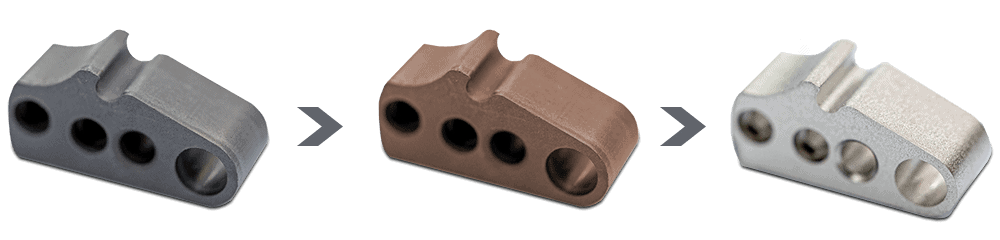
\includegraphics[width=0.8\linewidth]{bilder/img_gruenteil-braunteil-sinterteil.png}
        \caption[Der gesamte Prozess der Metallteilherstellung an einem Beispielteil dargestellt] {Der gesamte Prozess der Metallteilherstellung an einem Beispielteil dargestellt - von l. nach r. Grünteil; Braunteil, Sinterteil \autocite{junghans}}
	\label{fig:Prozess}
\end{figure}

In \autoref{fig:Prozess} ist der gesamte Prozess dargestellt. Links zu sehen ist das Bauteil, nachdem es aus dem 3D-Drucker entnommen wird. In der Mitte ist das entbundene Bauteil, in welchem der Polymer größtenteils gelöst und entfernt ist. Rechts im Bild zu sehen ist das Sinterbauteil, dies ist das fertige Bauteil.

\subsection{Arten des FDM-Verfahrens}
\label{sec:ArtenFDM}

FDM 3D-Drucker nutzen entweder einen Bowden-Extruder, oder einen Direktantrieb. Das Grundprinzip ist identisch, bei beiden Systemen fördert ein Elektromotor das Filament zum Hotend und damit zur Druckdüse. Die Verbindung von Elektromotor und Antriebsrad für das Filament wird Extruder genannt. Der Unterschied beider Verfahren ist die Lage dieses Extruders.

\begin{figure}[h]
	\centering
	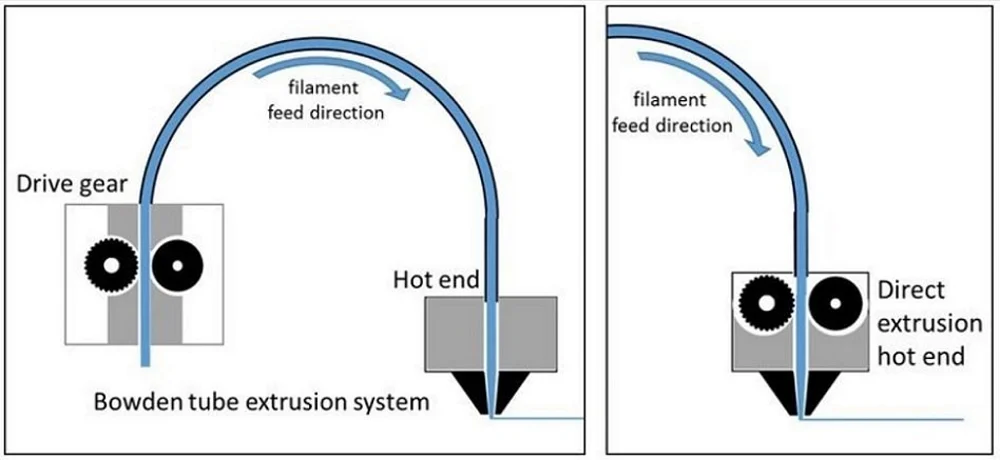
\includegraphics[width=0.8\linewidth]{bilder/img_BowdenvsDrirect.png}
        \caption[Schematische Darstellung von Bowden-Antrieb (links) und Direktantrieb (rechts)] {Schematische Darstellung von Bowden-Antrieb (links) und Direktantrieb (rechts) \autocite{facfox}}
	\label{fig:Verfahren}
\end{figure}

Wie in \autoref{fig:Verfahren} dargestellt, sitzt der Extruder beim Bowden-Extruder weit hinter der Düse. Das Filament wird vom Extruder durch einen Polytetrafluorethylen-Schlauch \textit{(PTFE)} und zum heißen Heizblock \textit{engl. Hotend} gedrückt. In dem Heizblock befindet sich die Druckdüse, durch die das aufgeheizte Filament extrudiert wird. Beim Direktextruder hingegen ist der Extruder unmittlebar vorm Hotend befestigt, dadurch wird das Filament vom PTFE-Schlauch direkt in den Extruder gepresst. Die Vor- und Nachteile sind hier aufgelistet:

\subsection*{Vorteile Direktextruder:}
\begin{itemize}
    \item Weniger Extrusionsprobleme: Der Extruder kann das Filament direkt zum Hotend fördern und muss es nicht durch ein Schlauch drücken.
    \item Kleinerer Motor notwendig: Aufgrund des kürzeren Abstands zwischen Extruder und Hotend wird weniger Drehmoment vom Motor benötigt.
    \item Mehr Auswahl an Filamenten: Sprödere Materialien, wie zum Beispiel Metallfilamente lassen sich drucken.
    \item Verbesserter Rückzug: der Extruder kann das Filament leichter zurückziehen, da er direkt über dem Hotend verbaut ist.
\end{itemize}

\subsection*{Nachteile Direktextruder:}
\begin{itemize}
    \item Höheres zu bewegendes Gewicht: Da der Extruder direkt am Druckkopf befestigt ist, muss er allen Bewegungen des Druckkopfes folgen. Dies sorgt für schlechtere dynamische Eigenschaften und Vibrationen
    \item Aufwändigere Wartung: Der Extruder ist am Druckkopf befestigt, welches eventuelle Wartungsarbeiten erschwert.
\end{itemize}

Für den Antrieb nach dem Bowden-Prinzip ergeben sich genau gespiegelte Vor- und Nachteile. \autocite{facfox}

\subsection{Lineare Vorschubtechnik}
\label{sec:LineareVorschub}

Die Lineare Vorschubregelung \textit{(engl. linear advance)}, ist eine Technik, die darauf abzielt, die Druckqualität und Geschwindigkeit beim FDM-Druck zu verbessern. Es sich dabei um einen algorithmischen Ansatz, der die Materialzufuhr während des Druckens in Echtzeit optimiert. Durch die Berücksichtigung der variablen Geschwindigkeiten und Beschleunigungen des Druckkopfes ermöglicht die Lineare Vorschubregelung eine präzisere Steuerung des Filamentflusses.
Die Lineare Vorschubregelung basiert auf der Idee, dass die Materialzufuhr nicht statisch ist, sondern dynamisch an die Bewegungen des Druckkopfes angepasst wird. Dieser Algorithmus betrachtet die Geschwindigkeitsänderungen des Druckkopfes und passt den Filamentvorschub linear an. Dies führt zu einer Reduzierung von Druckartefakten wie Überextrusion in Kurven oder Unterextrusion in geraden Abschnitten. \autocite{prusaLinearAdvance}

\begin{figure}[h]
	\centering
	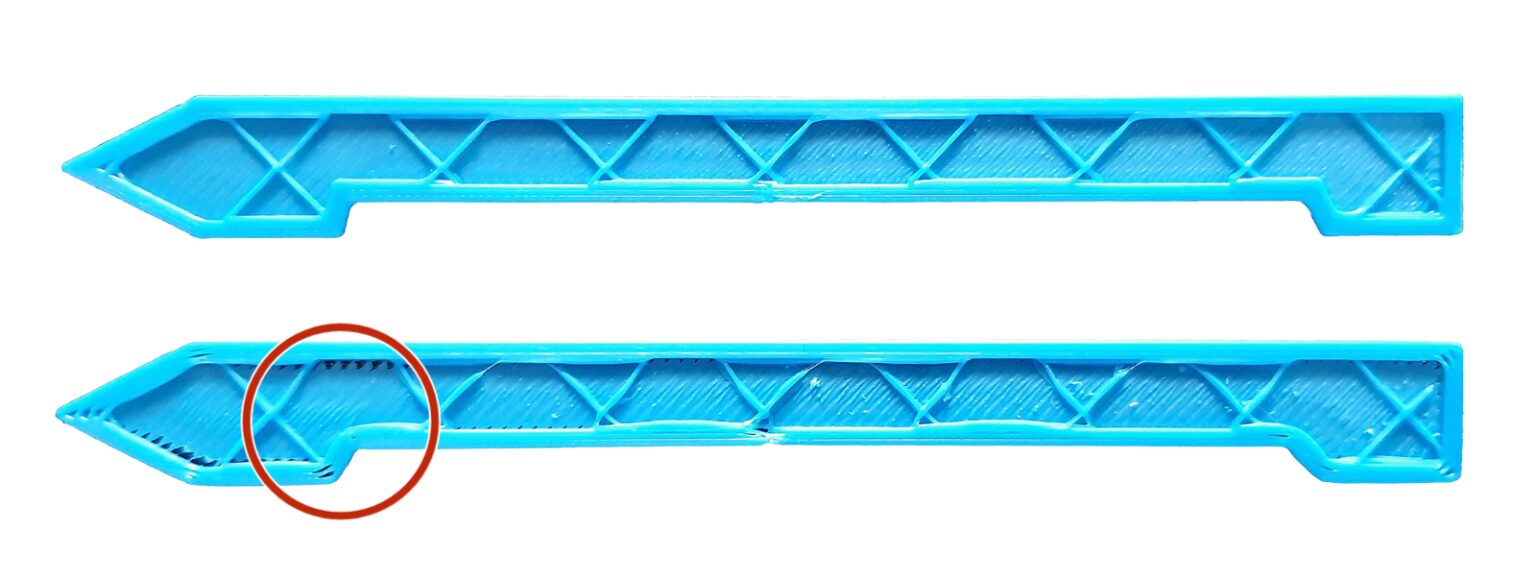
\includegraphics[width=0.8\linewidth]{bilder/img_linear-advance.jpeg}
        \caption[Darstellung lineare Vorschubregelung] {Darstellung lineare Vorschubregelung - oben: gutes Druckergebnis; unten: Artefakte durch falsche Einstellung von linearer Vorschubregelung \autocite{prusaLinearAdvance}}
	\label{fig:linearadvance}
\end{figure}
\chapter{Experimenteller Aufbau}

In diesem Kapitel wird darauf eingegangen, wie die Proben erstellt werden, welche Druckparameter eine große Rolle Spielen und wie diese gefunden werden. Ausserdem wird erklärt, welche Messverfahren und welche Messgeräte eingesetzt werden.\\


\section{Auswahl der Druckparameter}

Beim verwenden eines 3D-Druckers ist es notwendig die Druckparameter passend zum gewünschten Ergebnis auszuwählen. Hierbei kommt es auf die gewünschte Geometrie der späteren Bauteile und auf das verwendete Material an. Im Vorfeld dieser Arbeit ist bereits eine Wissenschaftliche Arbeit zum Thema \glqq FDM-Druck mit PT+A 316L Metallfilament Untersuchung der Druckparameter am Raise 3D Pro 2\grqq erstellt. Das Ergebnis dieser Arbeit lässt sich in Tabelle aus \autoref{ursprüngliche Werte} darstellen.

\begin{table}[htbp]
    \centering
    \caption{Druckparameter - gegeben aus \autocite{M.Mickan}}
      \begin{tabular}{llr}
      \toprule
      \textbf{Slicing-Paramater} & \textbf{Empfehlung} & \multicolumn{1}{l|}{\textbf{Hinweise (IdeaMaker)}} \\
      \midrule
      Drucktemperatur & 130°C & \multicolumn{1}{p{12.555em}}{+- 5 °C möglich} \\
      Druckgeschwindigkeit & 30-60 mm/s & \multicolumn{1}{p{12.555em}}{Füllung schnell, Konturen langsam} \\
      Heizbetttemperatur & 40 °C & \multicolumn{1}{p{12.555em}}{Gute Ablösung und Schichthaftung} \\
      Rückzugsgeschwindigkeit & 20 mm/s & \multicolumn{1}{p{12.555em}}{0,5 mm Rückzugsmenge} \\
      Materialflussrate & \multicolumn{1}{r}{90\%} & \multicolumn{1}{p{12.555em}}{Bei Extrusionsbreite 0,4 mm} \\
      Füllflussrate & \multicolumn{1}{r}{90\%} & \multicolumn{1}{p{12.555em}}{Vorsicht: Reiter „Fortgeschritten“ überschreibt Flussrateneinstellungen} \\
      Xy-Größenkompensation für Konturen & 0,1 mm &  \\
      Xy-Größenkompensation für Bohrungen & 0,06 mm &  \\
      Füllüberlappung & \multicolumn{1}{r}{10\%} & \multicolumn{1}{p{12.555em}}{Höher falls Ghosting / Pillowing eintritt} \\
      Schichthöhe & 0,3 mm &  \\
      \bottomrule
      \end{tabular}%
    \label{ursprüngliche Werte}%
  \end{table}%
  
Essentielle Parameter werden in dieser Arbeit jeweils mit Testdrucken bestimmt. Zur Bestimmung der Drucktemperatur wird ein sogenannter \textit{Heat Tower} gedruckt. Dabei wird in bestimmten Abständen die Temperatur in 5°C-Schritten abgesenkt. Mit dem gedruckten Bauteil lässt sich dann die geeigneteste Temperatur ablesen. \Autocite{M.Mickan}.\\

Diese Werte werden somit zu Beginn dieser Arbeit übernommen und erste Druckversuche werden durchgeführt. Dazu wird ein Würfel mit einer Kantenlänge von 10mm gewählt. Das Ergebnis ist in \autoref{erster Druck - Isometrie} und \autoref{erster Druck - Seitenansicht} dargestellt.


\begin{figure}[h]
	\centering
	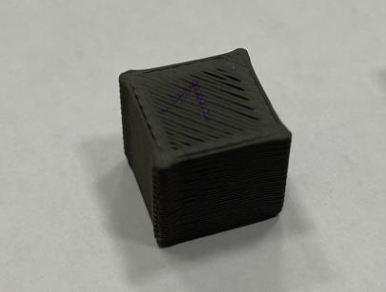
\includegraphics[width=0.5\linewidth]{bilder/Testdruck auf Raise Pro 3D.png}
        \caption[Testdruck von dem Raise3D Pro2 Plus - Isometrische Ansicht] {Testdruck von dem Raise3D Pro2 Plus - Isometrische Ansicht (Eigene Darstellung)}
	\label{erster Druck - Isometrie}
\end{figure}
\begin{figure}[h]
	\centering
	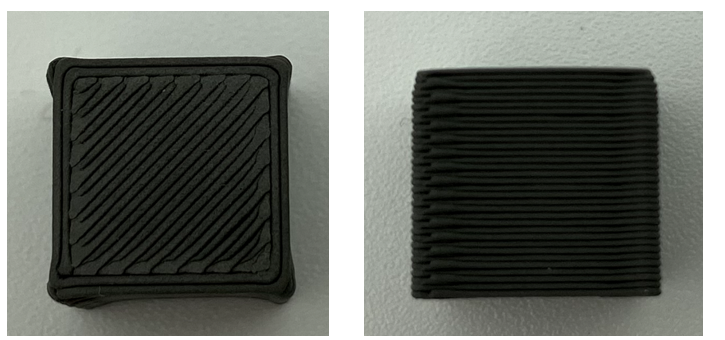
\includegraphics[width=\linewidth]{bilder/Testdruck auf Raise Pro 3D Seitenansicht - Draufsicht.png}
        \caption[Erster Testdruck mit dem Raise3D Pro2 Plus - Seitenansicht und Draufsicht] {Erster Testdruck mit dem Raise3D Pro2 Plus -Draufsicht (l) und Seitenansicht (r) (Geschwindigkeit: 60mm/s; Schichthöhe: 0,4mm) (Eigene Darstellung)}
	\label{erster Druck - Seitenansicht}
\end{figure}

Erkennbar ist hier deutlich, die ungenauigkeit des Drucks dargestellt. Dies lässt sich sehr gut in \autoref{erster Druck - Seitenansicht} an den Ecken in der rechten Draufsicht erkennen. Das Symptom der zu stark abgerundeten Ecken ist auf das Fehlen von \textit{linear advanced} aus \autoref{linear advanced} zurückzuführen. Die Extrusionsrate ist nicht an das Be- und Entschleunigungsverhalten des Druckkopfs angepasst. Dadurch ist an den Ecken, in denen die Geschwindigkeit langsamer ist, mehr Material aufgetragen. Die Einstellung des \textit{linear advanced} lässt sich bei diesem Drucker nicht einstellen und die \textit{Firmware} ist nicht \textit{Open Source}.

Bei Verringerung der Geschwindigkeit von 60mm/s auf 20mm/s ist dieser Effekt deutlich verringert. In \autoref{zweiter Druck - Isometrie} ist das Ergebnis der Verringerung der Geschwindigkeit und der Schichthöhe dargestellt. Doch diese Optimierung geht zu Lasten der gesamten Druckzeit. \textbf{HIER DieIE DRUCKZEIT BEREHCNEN!!}

\begin{figure}[h]
	\centering
	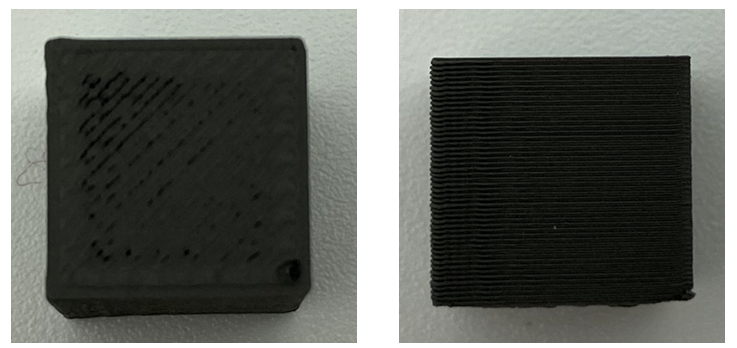
\includegraphics[width=\linewidth]{bilder/2. Testdruck auf Raise Pro 3D Seitenansicht - Draufsicht.png}
        \caption[Zweiter Testdruck mit dem Raise3D Pro2 Plus - Isometrische Ansicht] {Zweiter Testdruck mit dem Raise3D Pro2 Plus -Draufsicht (l) und Seitenansicht (r) (Geschwindigkeit: 20mm/s; Schichthöhe: 0,1mm) (Eigene Darstellung)}
	\label{zweiter Druck - Isometrie}
\end{figure}

\subsection{Verwendung des Prusa i3 MK3S+}
\label{Drucker}

Mit dem Raise 3D Pro 2 sind die Ergebnisse aufgrund der fehlenden Einstellmöglichkeit des \textit{linear advanced} nicht zufriedenstellend. Da auch die verlängerte Druckzeit bei verringerter Geschwindigkeit nicht zufriedenstellend ist, wird in dieser Arbeit auf den \textit{i3 MK3S+} der Frima \textit{Prusa} zurückgegriffen. Dieser hat ebenfalls wie der \textit{Raise3D}-Drucker einen Druckkopf mit Direktextruder. Dies ist vom Filamenthersteller aufgrund des spröden Materials empfohlen.

\begin{figure}[h]
	\centering
	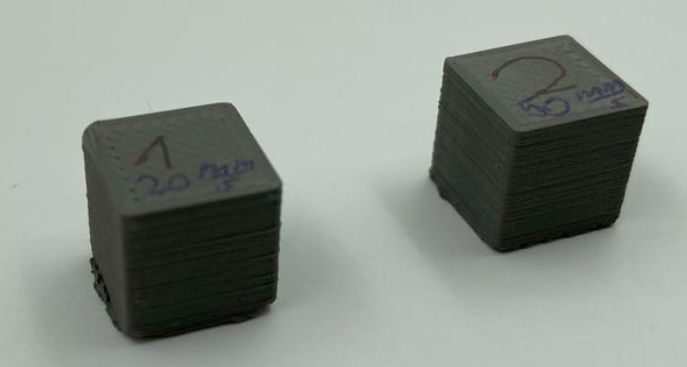
\includegraphics[width=\linewidth]{bilder/Erster Testdruck mit Prusa.png}
        \caption[Erster [20mm/s] und zweiter [50mm/s] Testdruck mit dem Prusa] {Erster [20mm/s] und zweiter [50mm/s] Testdruck mit dem Prusa (Eigene Darstellung)}
	\label{Erster Testdruck Prusa}
\end{figure}

Der erste Testdruck mit dem \textit{Prusa} ist in \autoref{Erster Testdruck Prusa} links dargestellt. Die Einstellungen gleichen den Einstellungen aus \autocite{M.Mickan}
(siehe \autoref{ursprüngliche Werte}). Die Geschwindigkeit ist jedoch auf 20mm/s reduziert und die Schichthöhe beträgt 0,1mm. Aufgrund des fehlerfreien Ergebnisses wird ebenso ein Würfel mit einer Geschwindigkeit von 50mm/s gedruckt. Dieser ist in \autoref{Erster Testdruck Prusa} rechts dargestellt. Somit stehen die Parameter für die Würfel und die liegenden Zugproben fest. Sie sind in \autoref{Würfelparameter} aufgefasst. 

\section{Probenherstellung und -messung}
Die Testwürfel sind in dem \textit{CAD}-System \textit{NX\textbf{VERSION??}} erzeugte Würfel mit einer Kantenlänge von 10mm. Diese sind dann als \textit{STL}-Datei exportiert und mit \textit{Ultimaker Cura Version 5.3.1} geslicet, also ein \textit{g-code} erzeugt. Wie bereits erwähnt wird für den Druck der \textit{Prusa MK3S+} mit einer \textbf{DÜSE??} verwendet. Auf dem originalen Druckbetts des \textit{Prusa} wird eine Schicht aus Flachkreppband der Marke \textit{Günter Seits \textbf{PRüfen!}} geklebt. Ohne dieses Flachkreppband haftet die erste Schicht zu gut an dem Druckbett, dadurch ist es unmöglich das Bauteil zerstörungsfrei von dem Druckbett zu lösen.\\
Die Würfel werden nun als Grünteil mit einem Digitalmessschieber der Marke \textit{Mitutoyo} gemessen. Die Proben werden einzeln mit einer \textit{Kern PRS 620-3} gewogen. Die Messwerte, samt errechntem Volumen und Dichte sind in \autoref{Grünteilmaße} aufgeführt.
\chapter{Ergebnisse und Diskussion}

4.1 Dichteauswertung der gedruckten 316L-Proben\\
4.1.1 Auswertungsmethoden und -ergebnisse\\
4.1.2 Einfluss der Druckparameter auf die Dichte\\
4.2 Schwindungsauswertung der gedruckten 316L-Proben\\
4.2.1 Auswertungsmethoden und -ergebnisse\\
4.2.2 Einfluss der Druckparameter auf die Schwindung\\
4.3 Vergleich mit theoretischen Werten oder Referenzproben\\
4.4 Diskussion der Ergebnisse
\chapter{Schlussfolgerungen}
\section{Zusammenfassung der Ergebnisse}

In dieser Arbeit werden die Ergebnisse der Untersuchungen zu Dichteeigenschaften und Schrumpfverhalten des 316L-Edelstahls durch FDM-Druck präsentiert und diskutiert. Die Dichte der gedruckten Proben wurde in den verschiedenen Prozessphasen analysiert, wobei eine durchschnittliche Dichte von 6,87 \(\text{g/cm}^3\) im Stahlteil erreicht wird. Die Schrumpfung des Volumens war, wie zu erwarten, besonders hoch im Sinterprozess.

Die Ergebnisse der Zugversuche zeigen Unterschiede zwischen den liegenden und stehenden Zugproben. Die stehenden Zugproben weisen gegenüber den liegend gedruckten, eine geringere Zugfestigkeit auf. Aufgrund von Schwierigkeiten bei den stehenden Zugproben konzentriert sich die Analyse auf die liegenden Proben. Die mechanischen Kennwerte, einschließlich Streckgrenze (R${\textsubscript{p0.2}}$), Zugfestigkeit (R${\textsubscript{m}}$) und Bruchdehnung (A$_{\textsubscript{25 mm}}$), werden ermittelt und mit Werkstoffdatenblattwerten für 1.4404 Edelstahl verglichen.
Die durchschnittliche Dichte wies eine Abweichung von -14\% im Vergleich zum Datenblatt auf. Ein Vergleich mit anderen Studien zeigte eine Abweichung von -10\%, wobei jedoch unterschiedliche Materialien und eine Druckdüse mit einem Durchmesser von 0,6mm verwendet werden. Insgesamt bieten diese Erkenntnisse Einblicke in die Druckqualität und ermöglichen mögliche Optimierungsansätze für zukünftige FDM-Druckprozesse mit 316L-Edelstahl. Zusätzlich befindet sich unter \autoref{Anleitungen} eine Anleitung für den Umgang mit verstopftem Hotend. Auch bietet die Anleitung einen Einstieg in den Druck mit Metallfilament. Inspiration ist die offizielle Anleitung aus \Autocite{Prusa}, doch sie ist optimiert auf das Drucken mit Metallfilament.

\section{Ausblick}

Um die Dichte zu verbessern, wurde in \autocite{Quarto.2021} eine Düse mit einem Durchmesser von 0,6 mm verwendet, was zu einer Dichte von knapp über 7,2 \(\text{g/cm}^3\) führte. Daher ist es sinnvoll weitere Versuche mit verschiedenen Düsendurchmessern anzustellen. Zusätzlich können Schrumpfungseffekte durch Messungen an größeren Würfeln analysiert werden. Dies ermöglicht Rückschlüsse auf das Verhalten des Polymers bei größeren Volumina. Interessant sind Vergleiche bei der Schrumpfung der Masse. Da es schwieriger ist, das Polymer aus dem Inneren von größeren Bauteilen zu entfernen.
Ebenfalls interessant ist es den Druck von stehenden Zugproben zu optimieren. 
Das Unternehmen \textit{PT+A} bietet verschiedene Materialien an. Es ist ebenfalls sinnvoll mit der Absprache mit diesem Unternehmen, auch Versuche mit verschiedenen Materialien durchzuführen.\\
Des Weiteren ist es ebenfalls interessant, wie das Verfahren des Metalldrucks in der Industrie integriert werden kann. Hier bedarf es an Forschung nach Möglichkeiten.
\let\cleardoublepage\clearpage

%% ...
%%\chapter{Diskursiver Teil}
\label{Zusammenfassung}



%% Beginn vom Anhang ------------------------------------------------------------------------------
\appendix

%% Literaturverzeichnis einbinden. Die Quellen sind in der Datei "LiteraturDB.bib" gespeichert. ---
%% Das Literaturverzeichnis muss vorab über über Tools-->Befehle-->Biber erzeugt werden.--
\begin{flushleft}  % Schaltet den Blocksatz für das Literaturverzeichnis ab.
     \printbibliography
\end{flushleft}
%% Anhang einbinden -------------------------------------------------------------------------------
\chapter{Anhang}
\label{Anhang}

\section{Druckparameter}

\begin{table}[htbp]
    \centering
    \caption{Parametertabelle Prusa MK3S+\newline verwendet für Druck der Würfel und liegenden Zugproben}
      \begin{tabular}{llr}
      \toprule
      \textbf{Parameter} & \textbf{Wert} & \multicolumn{1}{l}{\textbf{Beschreibung}} \\
      \midrule
      Schichthöhe [mm] & \multicolumn{1}{r}{0,1} &  \\
      Drucktemperatur [°C] & \multicolumn{1}{r}{130} &  \\
      Druckgeschwindigkeit [mm/s] & \multicolumn{1}{r}{50} & \multicolumn{1}{p{12.555em}}{Liefert optisch gute Ergebnisse} \\
      Heizbetttemperatur [°C] & \multicolumn{1}{r}{40} &  \\
      Rückzugslänge [mm] & \multicolumn{1}{r}{0,6} & \multicolumn{1}{p{12.555em}}{Standardwert Cura} \\
      Materialflussrate [\%] & \multicolumn{1}{r}{100} &  \\
      Druckoberfläche & Flachkreppband & \multicolumn{1}{p{12.555em}}{Gute Ablöseeigenschaften mit Spachtel} \\
      Prozentsatz Aussenhaut überlappen [\%/mm] & 10/0,04 &  \\
      \bottomrule
      \end{tabular}%
    \label{Würfelparameter}%
  \end{table}


\section{Messwerte}

\begin{table}[htbp]
    \centering
    \caption{Abmaße, Volumen, Gewicht und Dichte des Würfels als Grünteil}
      \begin{tabular}{lrrrrrrr}
      \toprule
      \textbf{Würfel:} & \multicolumn{1}{l}{\textbf{Z (Höhe) [mm]:}} & \multicolumn{1}{l}{\textbf{Länge1 [mm]:}} & \multicolumn{1}{l}{\textbf{Länge2 [mm]:}} & \multicolumn{1}{l}{\textbf{Gesamtvolumen [mm3]:}} & \multicolumn{1}{l}{\textbf{Gesamtvolumen [cm3]:}} & \multicolumn{1}{l}{\textbf{Gewicht [g]:}} & \multicolumn{1}{l}{\textbf{Dichte [g/cm3]}} \\
      \multicolumn{1}{r}{1} & 10,03 & 10,13 & 10,2  & 1036,36 & 1,0364 & 4,775 & 4,607 \\
      \multicolumn{1}{r}{1} & 10,01 & 10,12 & 10,2  & 1033,27 & 1,0333 & 4,765 & 4,612 \\
      \multicolumn{1}{r}{1} & 10,02 & 10,15 & 10,17 & 1034,32 & 1,0343 & 4,76  & 4,602 \\
      \multicolumn{1}{r}{1} & 10,04 & 10,14 & 10,19 & 1037,40 & 1,0374 & 4,761 & 4,589 \\
      \multicolumn{1}{r}{1} & 10,03 & 10,15 & 10,19 & 1037,39 & 1,0374 & 4,76  & 4,588 \\
      \multicolumn{1}{r}{1} & 10,05 & 10,15 & 10,14 & 1034,36 & 1,0344 & 4,768 & 4,610 \\
      \multicolumn{1}{r}{1} & 10,06 & 10,13 & 10,19 & 1038,44 & 1,0384 & 4,751 & 4,575 \\
      \multicolumn{1}{r}{1} & 10,03 & 10,16 & 10,16 & 1035,35 & 1,0354 & 4,763 & 4,600 \\
      \multicolumn{1}{r}{1} & 10,02 & 10,17 & 10,16 & 1035,34 & 1,0353 & 4,762 & 4,599 \\
      \textbf{Schnitt1:} & \textbf{10,03} & \textbf{10,14} & \textbf{10,18} & \textbf{1035,80} & \textbf{1,0358} & \textbf{4,7628} & \textbf{4,5982} \\
      \midrule
      \multicolumn{1}{r}{2} & 9,94  & 10,22 & 10,2  & 1036,19 & 1,0362 & 4,724 & 4,559 \\
      \multicolumn{1}{r}{2} & 10,01 & 10,2  & 10,22 & 1043,48 & 1,0435 & 4,731 & 4,534 \\
      \multicolumn{1}{r}{2} & 9,97  & 10,18 & 10,22 & 1037,27 & 1,0373 & 4,754 & 4,583 \\
      \multicolumn{1}{r}{2} & 9,93  & 10,16 & 10,18 & 1027,05 & 1,0270 & 4,741 & 4,616 \\
      \multicolumn{1}{r}{2} & 9,97  & 10,21 & 10,22 & 1040,33 & 1,0403 & 4,751 & 4,567 \\
      \multicolumn{1}{r}{2} & 9,95  & 10,21 & 10,22 & 1038,24 & 1,0382 & 4,737 & 4,563 \\
      \multicolumn{1}{r}{2} & 9,95  & 10,15 & 10,23 & 1033,15 & 1,0332 & 4,741 & 4,589 \\
      \multicolumn{1}{r}{2} & 9,94  & 10,21 & 10,17 & 1032,13 & 1,0321 & 4,738 & 4,591 \\
      \textbf{Schnitt2:} & \textbf{9,96} & \textbf{10,19} & \textbf{10,21} & \textbf{1035,98} & \textbf{1,0360} & \textbf{4,7396} & \textbf{4,5751} \\
      \bottomrule
      \end{tabular}%
    \label{Grünteilmaße}%
  \end{table}%
  
\section{Anleitungen}
\subsection*{Anleitung bei verstopftem Hotend/Druckdüse}

Sollten Schwierigkeiten bei der Extrusion des Metallfilaments auftreten, wie beispielsweise eine Blockade im Hotend oder der Druckdüse, erfordert dies jedes Mal eine Demontage des Extruders. In der Folge muss die Verstopfung im PTFE-Schlauchstück sorgfältig entfernt werden. Diese Anleitung orientiert sich an \Autocite{Prusa}, jedoch wird auf den Austausch des PTFE-Schlauchstücks verzichtet.
Hinweis: Diese Anleitung bezieht sich lediglich auf den verwendeten \textit{Prusa i3 MK3S+}.\\
Hinweis: Niemals heiße Bauteile mit den Händen berühren!
\begin{itemize}
  \item Folgende Werkzeuge werden benötigt:
    \begin{itemize}
      \item Spitzzange
      \item 2,5mm Imbussschlüssel
    \end{itemize}
    \item Das Heizbett wird mit einem dicken Tuch geschützt, sodass eventuelle Verunreinigungen oder herabfallende Maschinenelemente die Oberfläche nicht beschädigen. Die X-Achse wird auf die Hälfte der Gesamthöhe gefahren (siehe \autoref{X-Achse hoch}). Ebenso ist darauf zu achten, dass der Drucker vollständig heruntergekühlt ist und er wird vom Stromnetz genommen.
      \begin{figure}[h]
        \centering
        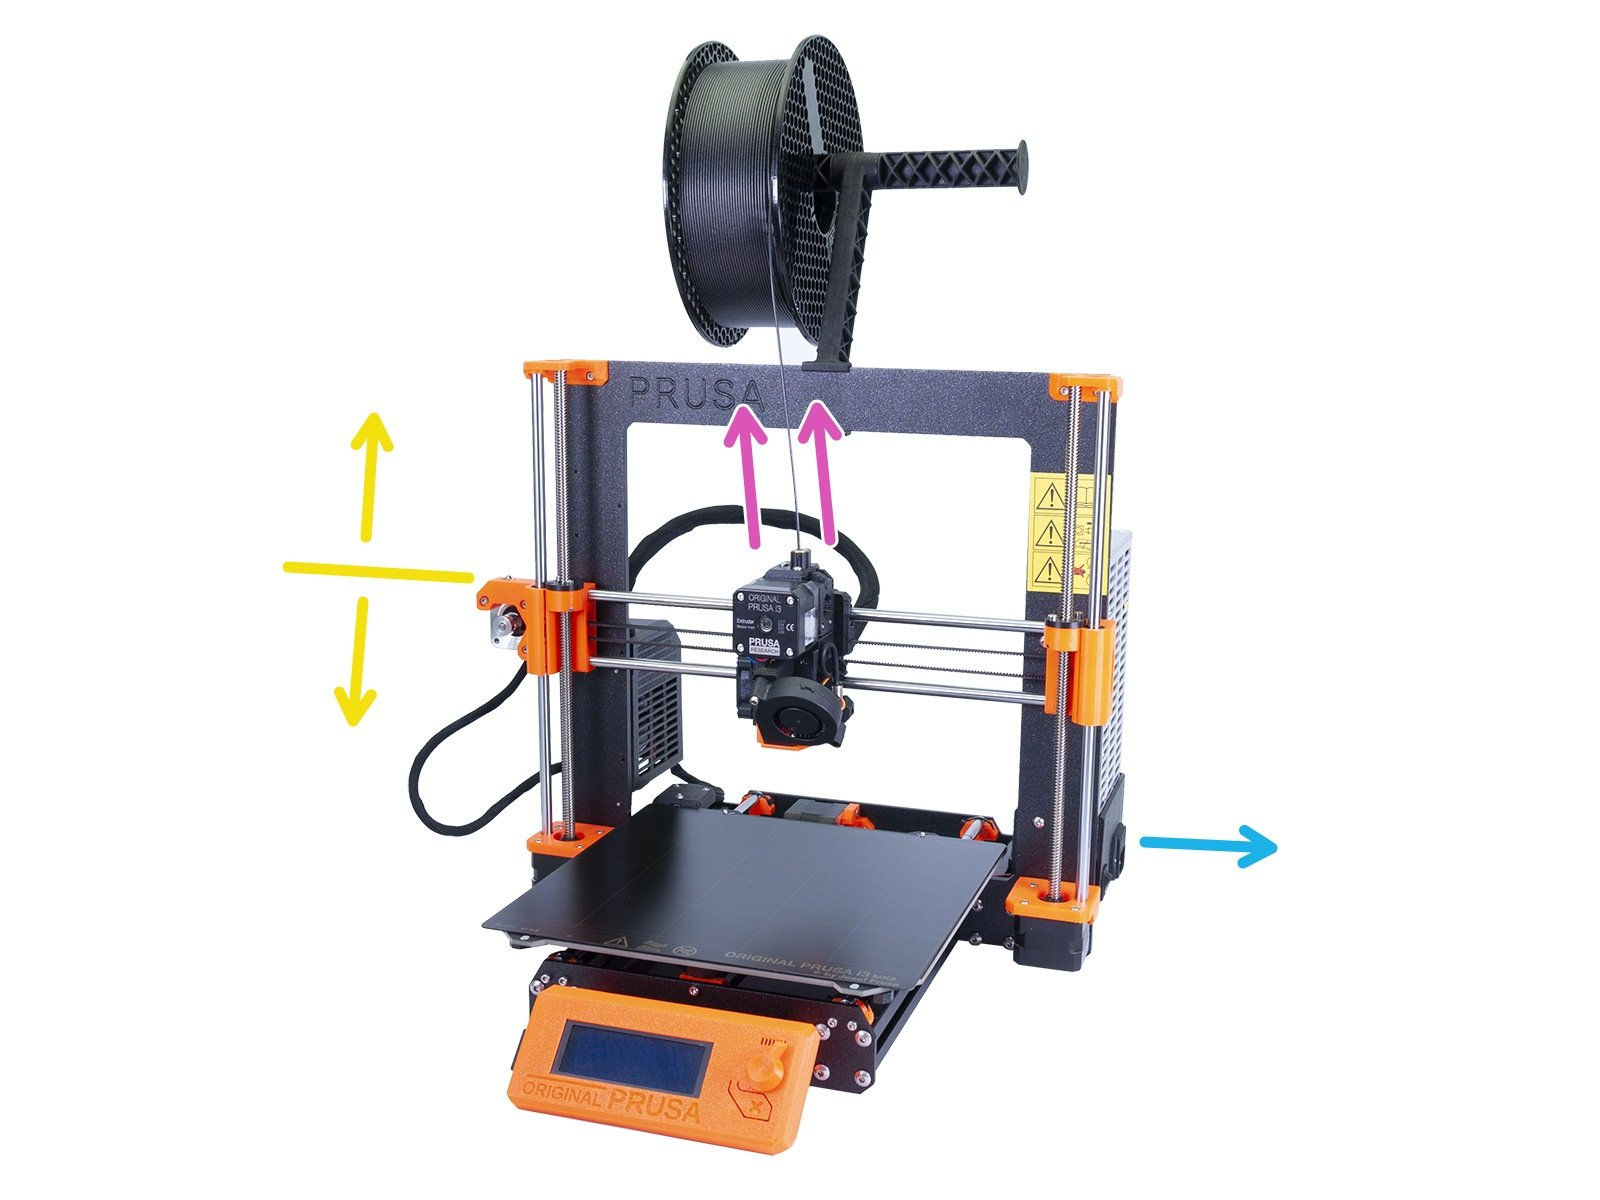
\includegraphics[width=0.5\linewidth]{bilder/Anleitung - X-Achse hoch.jpg}
              \caption[Anleitung: X-Achse auf die Hälfte der Gesamthöhe fahren] { X-Achse auf die Hälfte der Gesamthöhe fahren (Quelle: \autocite{Prusa})}
        \label{X-Achse hoch}
      \end{figure}
    \item Nun folgt das entfernen der Schrauben. Zunächst werden die in \autoref{Schraubi1} dargestellten Schrauben gelöst und entfernt. Im Anschluss werden die grün markierten Schrauben aus \autoref{Schraubi2} entfernt. Abschließend gilt es die orange markierten Schrauben, die den Extruder halten, aus \autoref{Schraubi3} zu entfernen.
      \begin{figure}[h] 
        \centering
        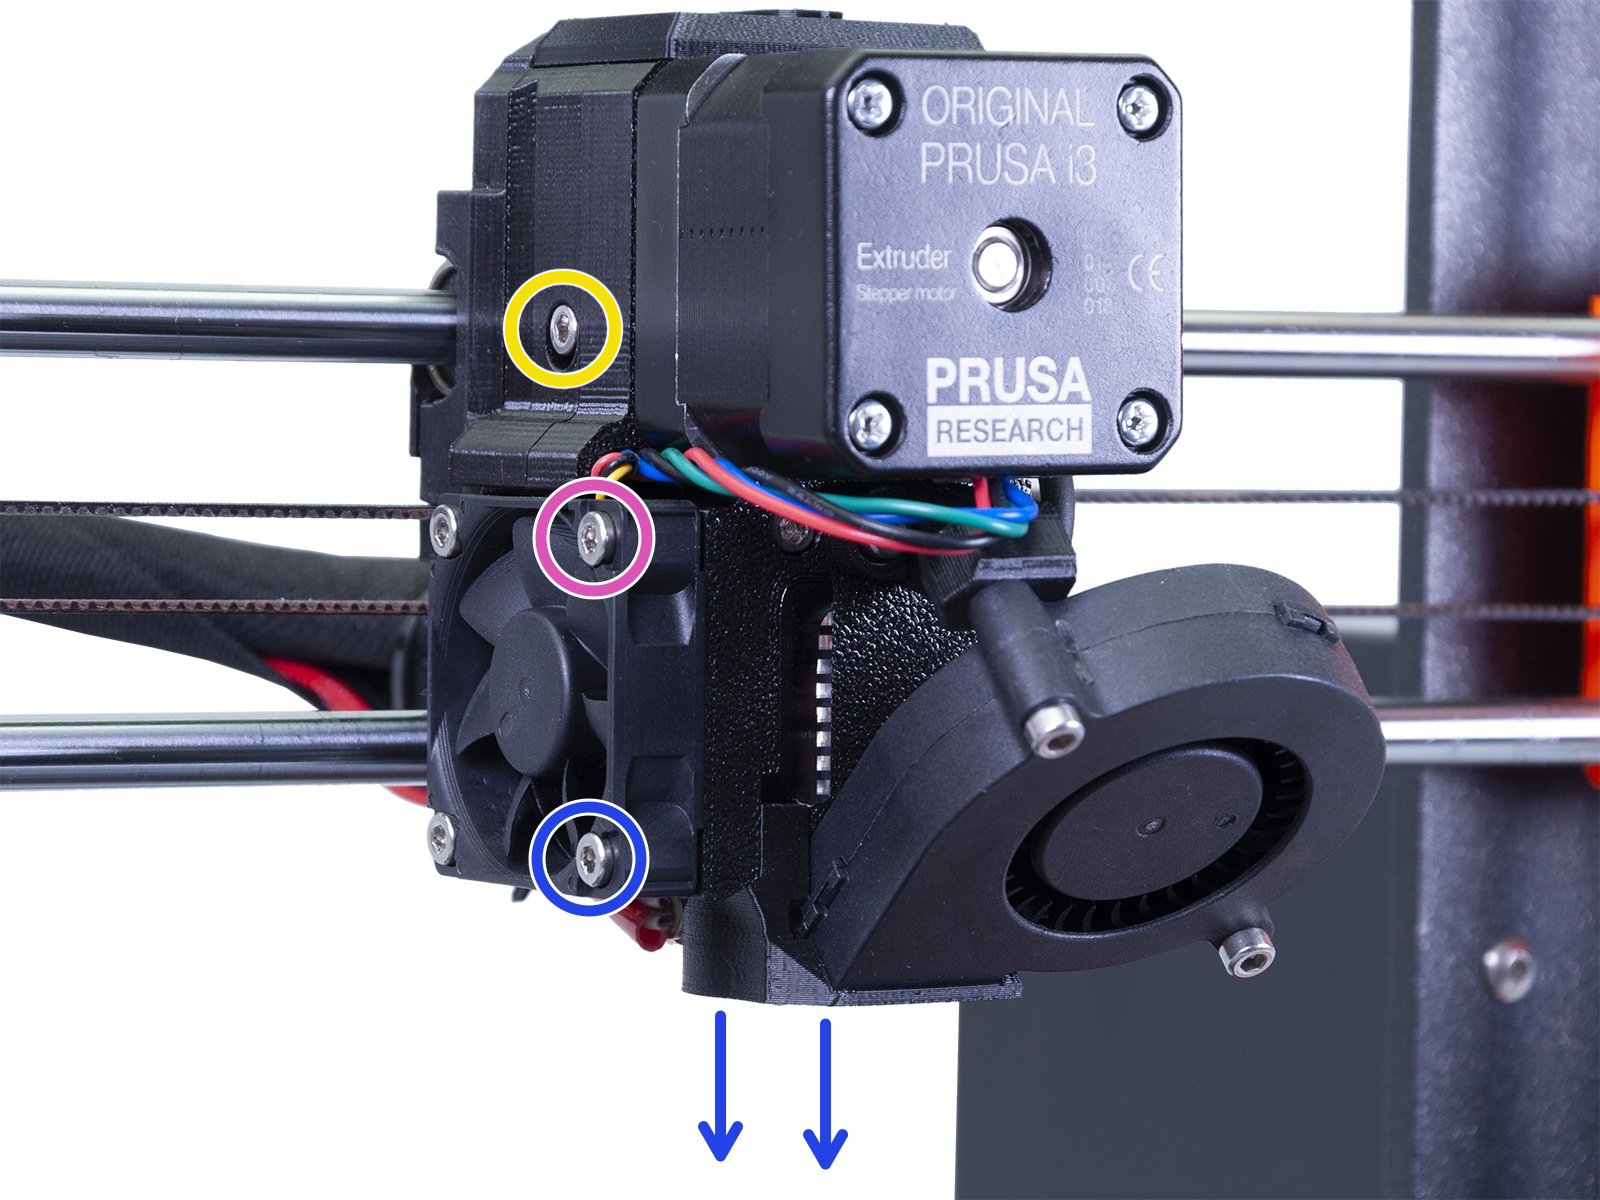
\includegraphics[width=0.5\linewidth]{bilder/Anleitung - Schraubi1.jpg}
              \caption[Anleitung: Gelb, lila und blau markierten Schrauben entfernen] {Gelb, lila und blau markierten Schrauben entfernen (Quelle: \autocite{Prusa})}
        \label{Schraubi1}
      \end{figure}
      \begin{figure}[h]
        \centering
        \begin{subfigure}[b]{0.45\textwidth}
          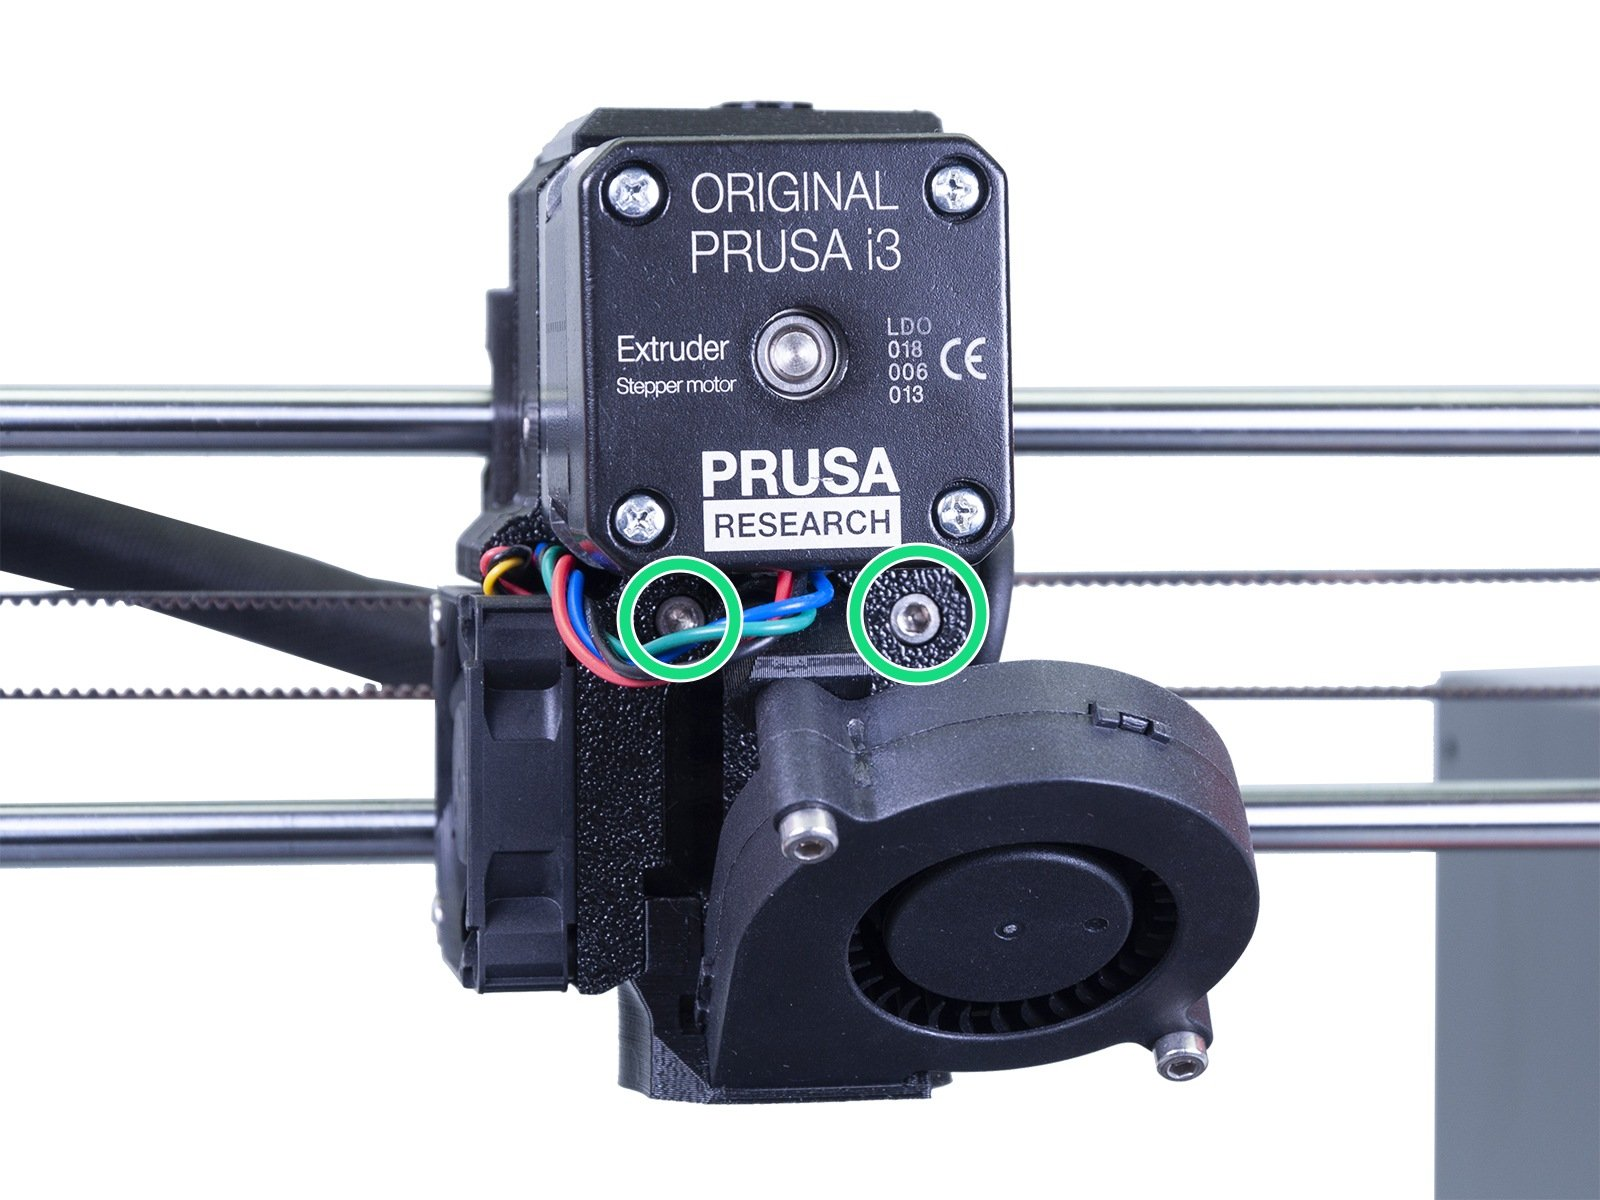
\includegraphics[width=\textwidth]{bilder/Anleitung - Schraubi2.jpg}
          \caption[Anleitung: Grün markierte Schrauben entfernen] {Grün markierte Schrauben entfernen (Quelle: \autocite{Prusa})}
          \label{Schraubi2}
        \end{subfigure}
        \hfill
        \begin{subfigure}[b]{0.45\textwidth}
          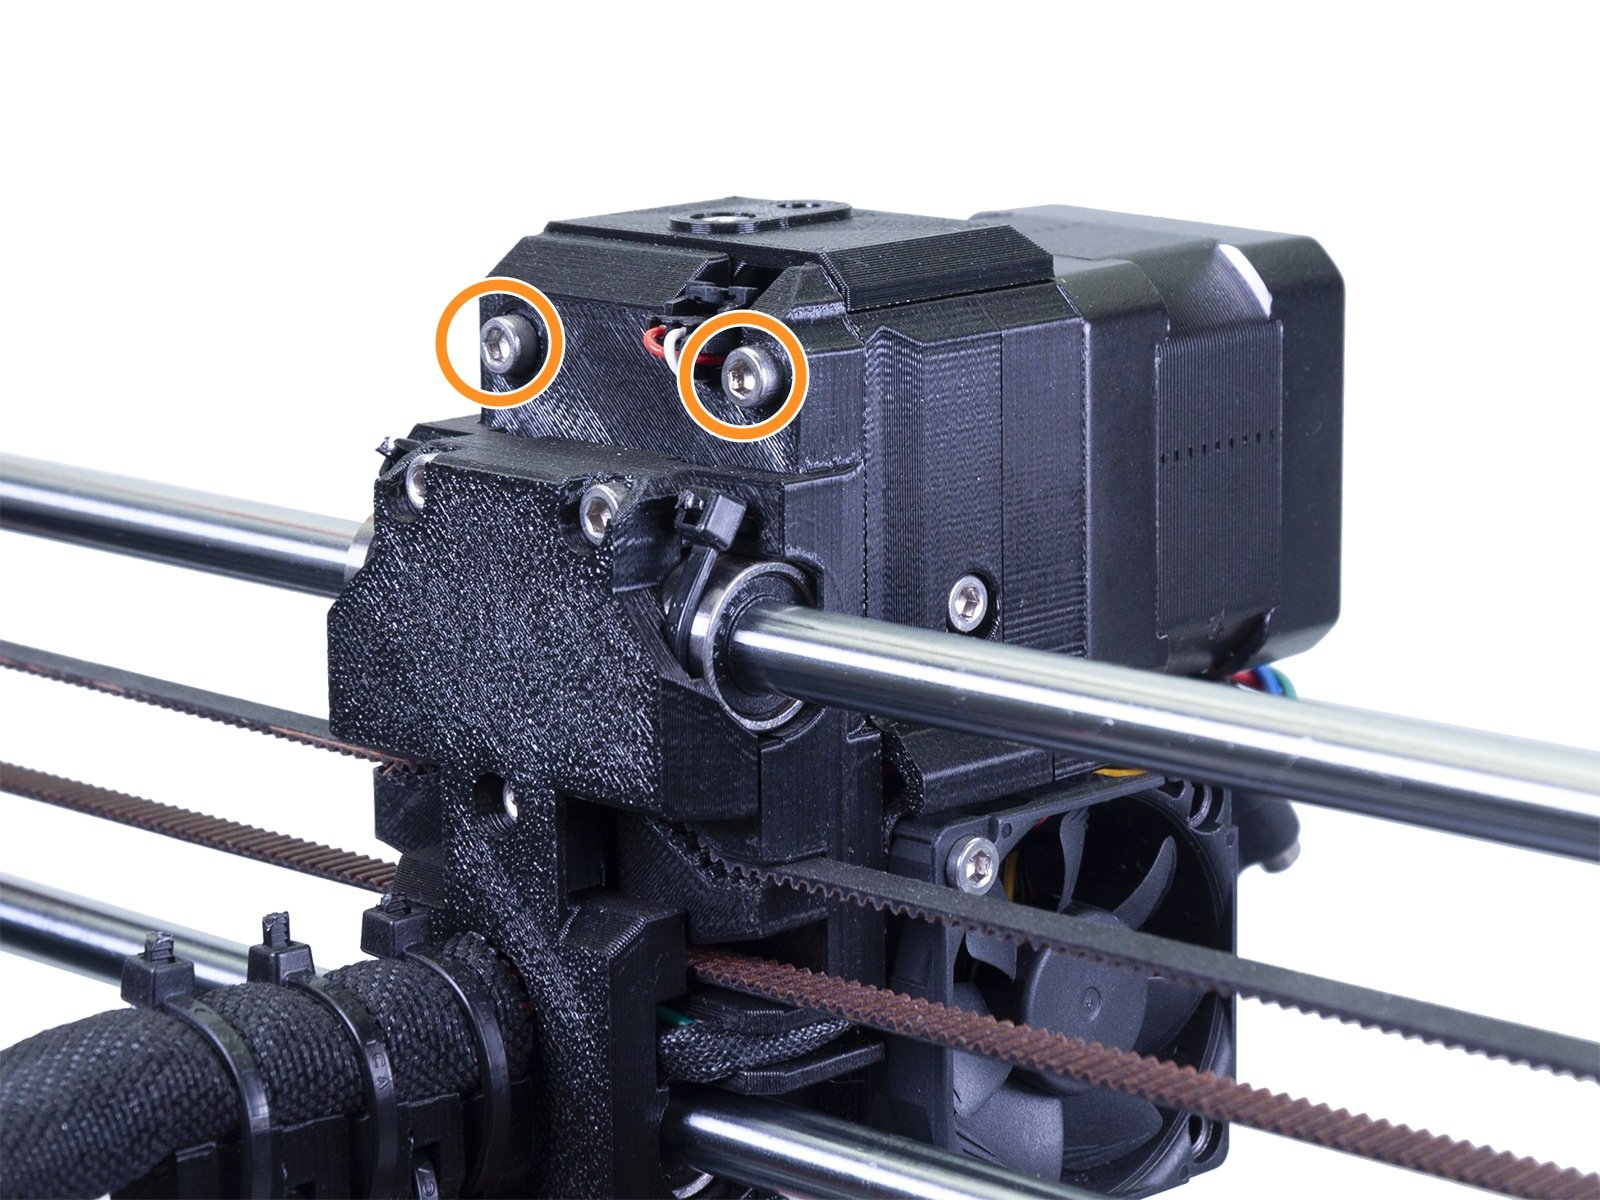
\includegraphics[width=\textwidth]{bilder/Anleitung - Schraubi3.jpg}
          \caption[Anleitung: Orange markierte Schrauben entfernen] {Orange markierte Schrauben entfernen (Quelle: \autocite{Prusa})}
          \label{Schraubi3}
        \end{subfigure}
      \end{figure}
    \item In diesem Schritt wird der Extruder teildemontiert. Dazu Wird vorsichtig der Extrudermotor in Pfeilrichtung (siehe \autoref{Zerlegen1}) gezogen. Sobald dieser lose ist, wird der untere Teil mit herausgezogen. Es muss eine Lücke, wie in \autoref{Zerlegen1} in gelb dargestellt, zu sehen sein.\\
          Nun kann das Hotend vorsichtig von unten entnommen werden (siehe \autoref{Zerlegen2}). Dabei auf die Kabel des Hotends achten, sie dürfen nicht beschädigt werden.
      \begin{figure}[h] 
        \centering
        
      \end{figure}
      \begin{figure}[h]
        \centering
        \begin{subfigure}[b]{0.45\textwidth}
          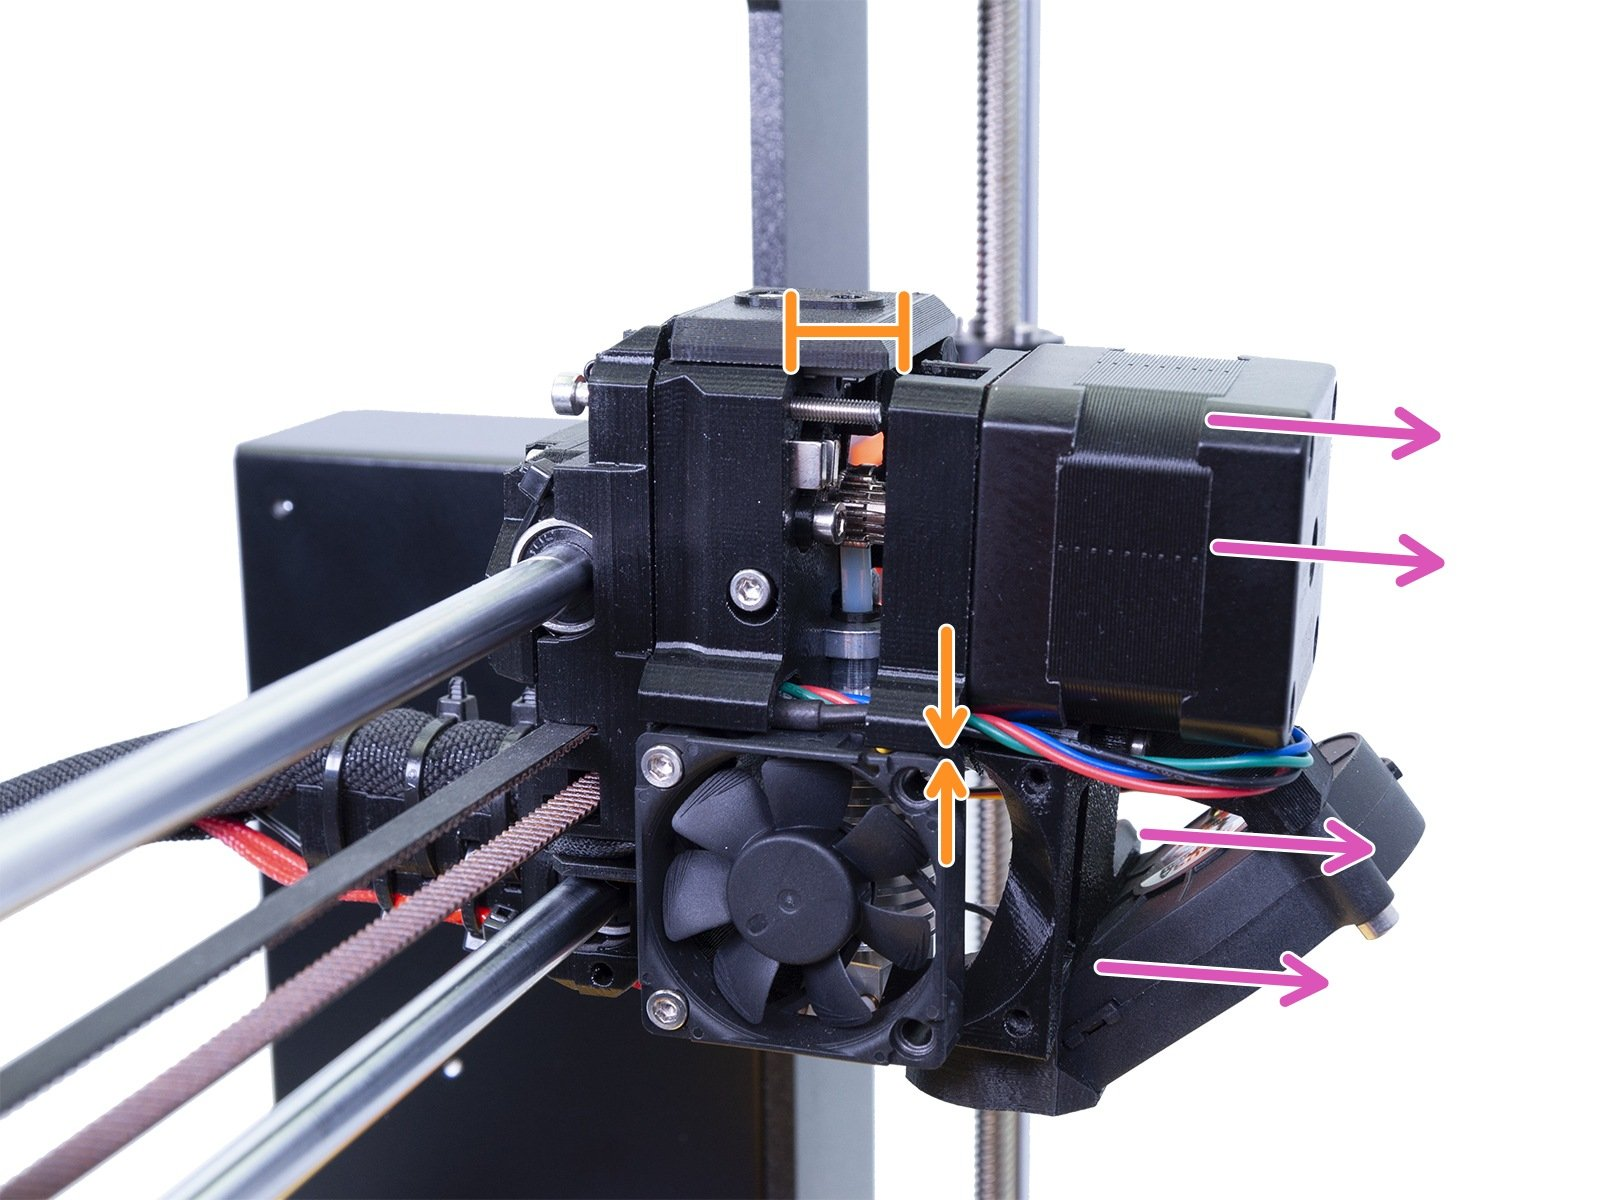
\includegraphics[width=0.5\linewidth]{bilder/Anleitung - Zerlegen1.jpg}
          \caption[Anleitung: Zerlegung des Extruders] {Zerlegung des Extruders (Quelle: \autocite{Prusa})}
        \label{Zerlegen1}
        \end{subfigure}
        \hfill
        \begin{subfigure}[b]{0.45\textwidth}
          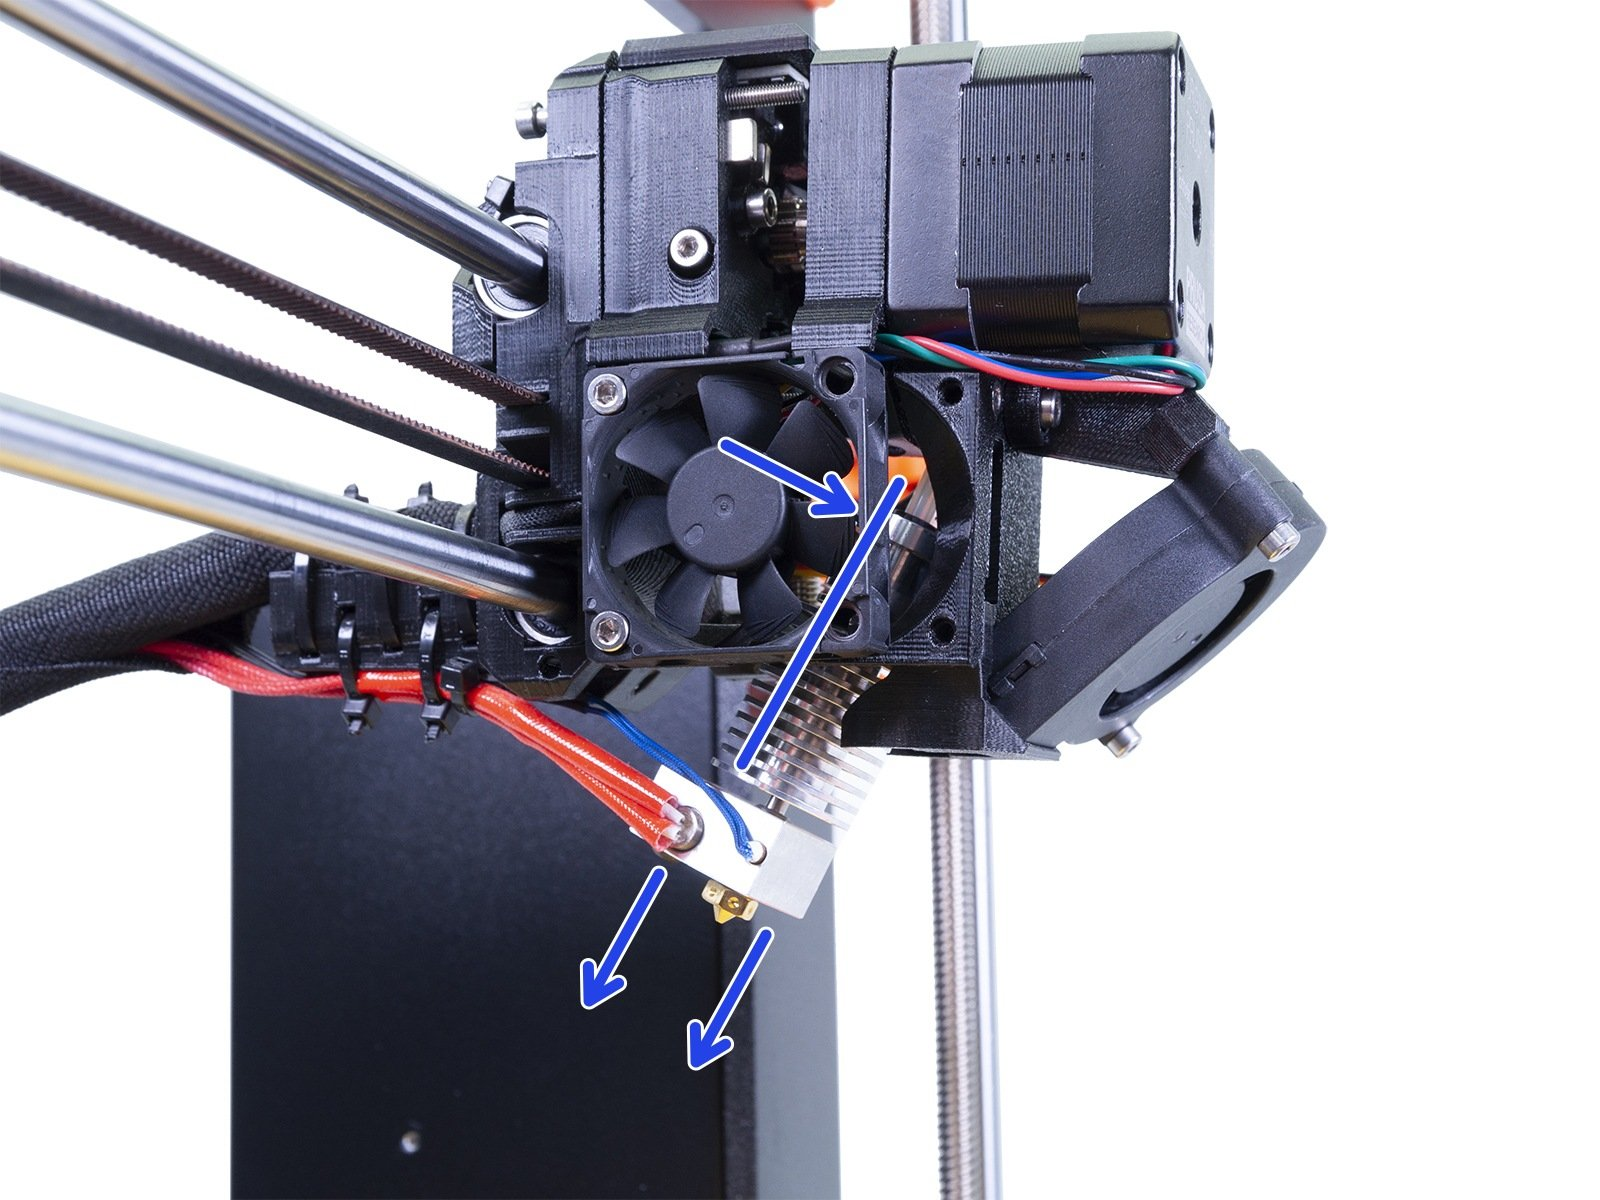
\includegraphics[width=\textwidth]{bilder/Anleitung - Zerlegen2.jpg}
          \caption[Anleitung: Vorsichtige Entnahme des Hotends] {Vorsichtige Entnahme des Hotends (Quelle: \autocite{Prusa})}
          \label{Zerlegen2}
        \end{subfigure}
      \end{figure}
    \item Jetzt kann das PTFE-Schlauchstück mithilfe der entfernt werden. Dazu mit den Fingern den, in \autoref{PTFEEE} mit blauem Pfeil markierten, Ring herunterdrücken und den Schlauch mit der beiliegenden Zange herausziehen. Nun kann die Verstopfung in diesem Schlauchstück mit einem langen, dünnen Hilfsmittel (z.B. einem Imbussschlüssel) entfernt werden.
      \begin{figure}[h] 
        \centering
        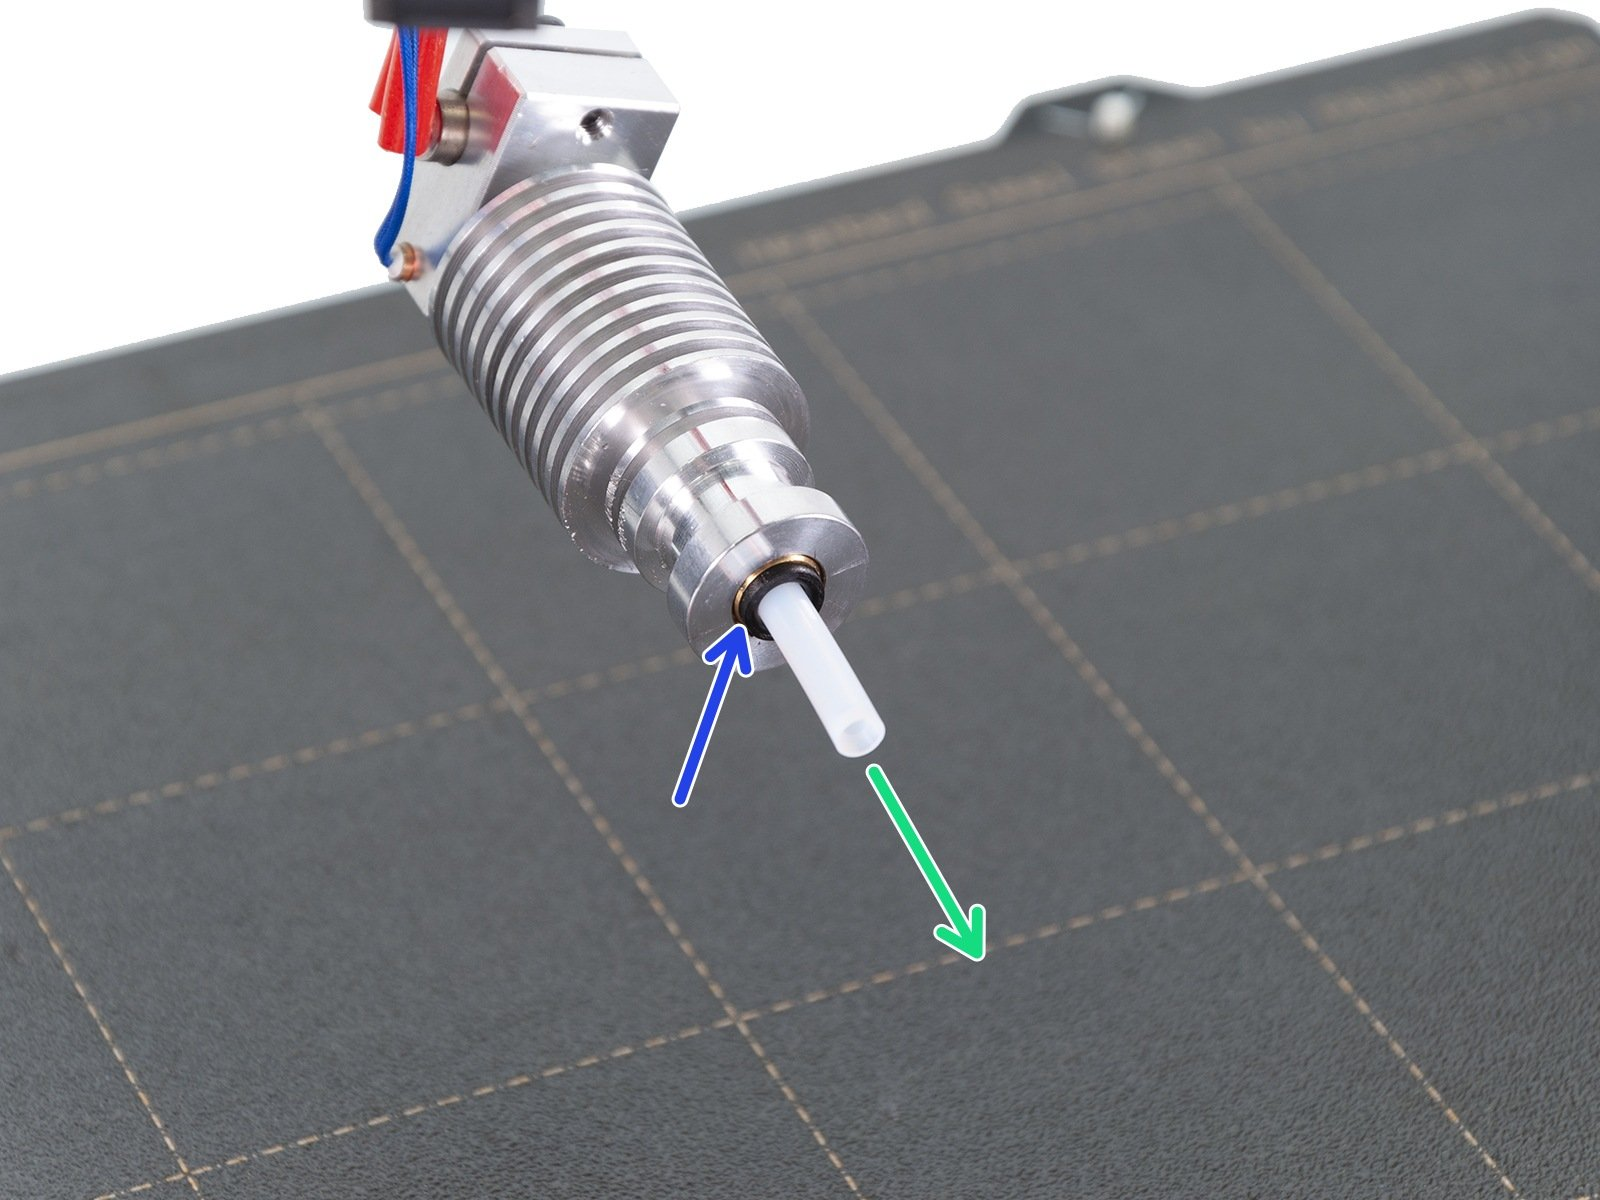
\includegraphics[width=0.5\linewidth]{bilder/Anleitung - Entfernen des PTFE-Schlauchs.jpg}
              \caption[Anleitung: Entfernen des PTFE-Schlauchstücks] {Entfernen des PTFE-Schlauchstücks (Quelle: \autocite{Prusa})}
        \label{PTFEEE}
      \end{figure}
    \item Der Zusammenbau geschieht in umgekehrter Reihenfolge. Wichtig ist, dass der PTFE-Schlauch mit dem angespitztem Ende wieder in den Extruder hineingeführt wird.
    \item Die in gelb dargestellte Schra
    \item Wenn alle Teile wieder zusammengebaut und die Schrauben wieder festgezogen sind, kann die Düse auf 180°C aufgeheizt werden. Sobald die Temperatur erreicht ist, wird das Ende der Filamentrolle schräg mit der Zange abgeschnitten. Um das  
\end{itemize}

\end{document}
